\documentclass[11pt,a4paper]{article}

\usepackage[margin=0.84in]{geometry}
\usepackage[T1]{fontenc}
\usepackage[utf8]{inputenc}
\usepackage{lmodern}
\usepackage{microtype}
\usepackage{amsmath,amssymb,amsthm,mathtools}
\usepackage{booktabs}
\usepackage{graphicx}
\usepackage{enumitem}
\usepackage[hidelinks,
  pdftitle={Exact-Fp/Z Cartier-Operator Boundary-Residue, Pin-Eigenvector, and Hinge-Shortening Certificates for Border VP != VNP},
  pdfauthor={Lluis Eriksson}
]{hyperref}

\newtheorem{theorem}{Theorem}[section]
\newtheorem{proposition}[theorem]{Proposition}
\newtheorem{lemma}[theorem]{Lemma}
\newtheorem{remark}[theorem]{Remark}

\newcommand{\QQ}{\mathbb{Q}}
\newcommand{\ZZ}{\mathbb{Z}}
\newcommand{\NN}{\mathbb{N}}
\newcommand{\FF}{\mathbb{F}}
\newcommand{\Res}{\operatorname{Res}}
\newcommand{\certschema}{\texttt{BORDER-VPVNP-CERT-1.0}}
\emergencystretch=3em
\sloppy

\title{\bfseries Exact-$\FF_p/\ZZ$ Cartier-Operator Boundary-Residue, Pin-Eigenvector, and Hinge-Shortening Certificates for Border $\mathsf{VP} \neq \mathsf{VNP}$}

\author{Lluis Eriksson\thanks{Independent researcher (Sweden). Manuscript licensed under CC-BY-4.0. Prepared with AI-assisted formal verification, code generation, and mathematical drafting (Google Antigravity). Code, zero-dependency Lean~4 proofs, and exact-$\FF_p/\ZZ$ certificates (MIT license): \url{https://github.com/lluiseriksson/border-vp-vnp-residue-certificates}.}}

\date{November 2026}

\begin{document}
\maketitle

\begin{abstract}
On November 23, 2026, OpenAI (\texttt{openai/math}) separated Valiant's algebraic complexity classes in the Zariski closure, proving $\mathsf{VNP} \not\subseteq \overline{\mathsf{VP}}$ over every field with border circuit lower bound $\exp(\Omega((\log n)^{5/4}))$ (Theorem~1.1). A central algebraic engine of the proof reads regular boundary values $z \in \FF_p$ from degenerating curves whose individual computation paths carry cancelling Laurent poles by applying the characteristic-$p$ Cartier operator $C_p$ (Sections~3--5, Lemmas~3.3, 5.1, and~5.2) to construct residue pin matrices $(\sum_\mu a_\mu W_\mu)\Omega = z\Omega$, combined with Definition~2.1 strict hinge shortening, Section~4 Cramer/Hadamard bit-length bounds, and batched query replay. Here we formalize and operationalize these exact algebraic laws in an $18$-theorem zero-dependency Lean~4 kernel (\texttt{v4.35.0}, $0$~\texttt{sorry}, $0$~\texttt{Classical.choice}, $0$~warnings) paired with a pure-stdlib zero-float verifier (\certschema{}). First, we machine-check the exact integer Frobenius additivity defects $((u+v)^p - u^p - v^p)/p$ for $p \in \{2,3,5\}$ and Fermat's little theorem on $\FF_3$ and $\FF_5$ (Lean~4 Theorems~1--5). Second, we formalize the structural Cartier index laws---residue preservation $p(-1) + (p-1) = -1$, injectivity, semilinear shift $C_p(t^{pm}\eta) = t^m C_p(\eta)$, annihilation of non-$(p{-}1) \pmod p$ exponents, cancelling-pole invariance, and Eq.~(5.1) $2\times 2$ residue pin eigenvector linearity (Lean~4 Theorems~6--12). Third, we prove strict hinge shortening and $t$-th tensor-power gap amplification, inductive batched query degree budgets, $2\times 2$ Cramer/Hadamard determinant entry bounds, $\exp((\log n)^{5/4})$ superpolynomial dominance $2^{u^5} > (2^{u^4})^k$, and homogeneous degree conservation (Lean~4 Theorems~13--18). Our verifier replays $16/16$ exact-$\FF_p/\ZZ$ certificates in $0.024$--$0.305\,\mathrm{ms}$ (certifying Cartier semilinearity across $p = 3\dots 29$ and boundary recovery under cancelling poles up to order $10$), cross-checks Frobenius/Cartier identities across primes, and rejects $54/54$ live adversarial attacks in $0.06\,\mathrm{s}$.
\end{abstract}

\section{Introduction}

Valiant's algebraic $\mathsf{VP}$ vs.\ $\mathsf{VNP}$ problem~\cite{valiant1979completeness} and its geometric border strengthening $\mathsf{VNP} \not\subseteq \overline{\mathsf{VP}}$ (central to Geometric Complexity Theory~\cite{mulmuley2001geometric}) ask whether Zariski-closure limits of polynomial-size arithmetic circuits can approximate $\mathsf{VNP}$ families. On November 23, 2026, OpenAI~\cite{openai2026vpvnp} (subsequently extended to the full hierarchy~\cite{openai2026hierarchy}) proved that over every field, degree-$n$ border circuits for an explicit universal-machine $\mathsf{VNP}$ family require $\exp(\Omega((\log n)^{5/4}))$ gates.

To replay degenerating circuits whose parameters $X_i(t)$ diverge as $t \to 0$ even while outputs $Y(X(t))$ converge to a regular boundary value $z \in \FF_p$, Section~5 of~\cite{openai2026vpvnp} invokes the characteristic-$p$ Cartier operator $C_p(\sum_j v_j t^j dt) = \sum_i v_{pi + p - 1}^{1/p} t^i dt$ (generalizing St\"ohr--Voloch~\cite{stohr1986weierstrass}). Because $A(t)^p - z = (A(t) - z)^p \in t^p \FF_p[[t]]$ vanishes to order $\ge p$ whenever $A(t)$ is regular with $A(0) = z \in \FF_p$, pairing $A^p$ against any test differential $\eta$ of pole order $\le p$ yields $\Res(A^p \eta) = z\Res(\eta)$ even when individual monomial paths carry arbitrary cancelling poles, enabling residue pin matrices $(\sum_\mu a_\mu W_\mu)\Omega = z\Omega$ (Eq.~5.1). We mechanize all $18$ underlying Frobenius, Cartier, pin-eigenvector, hinge-shortening, Hadamard, and superpolynomial laws in zero-dependency Lean~4 (\texttt{lean/BorderVPVNPResidues.lean}) and build a pure-stdlib zero-float verifier (\certschema{}, \texttt{src/cartier\_certifier.py}) auditing explicit witnesses across all four modes.

\section{Main Exact-\texorpdfstring{$\FF_p/\ZZ$}{Fp/Z} Cartier, Pin, and Hinge Theorems}\label{sec:results}

\subsection{Frobenius Additivity Defects, Fermat's Little Theorem, and Cartier Index Laws}

\begin{theorem}[Frobenius Defects, Fermat Identity, and Structural Cartier Laws]\label{thm:cartier}
\leavevmode
\begin{enumerate}[leftmargin=1.8em,itemsep=2pt]
  \item \textbf{Exact Integral Frobenius Defects and Fermat's Little Theorem:} Over $\ZZ$, $(u+v)^p - u^p - v^p$ is explicitly divisible by $p$ for $p \in \{2,3,5\}$ (mechanizing the integral correction polynomial $((U+V)^p - U^p - V^p)/p$ in Lemma~5.2 of~\cite{openai2026vpvnp}), and $a^p \equiv a \pmod p$ for all $a \in \ZZ$ at $p \in \{3, 5\}$, certifying $v^{1/p} = v$ on prime fields $\FF_p$ (Lean~4 Theorems~1--5).
  \item \textbf{Cartier Residue Preservation, Semilinearity, and Annihilation:} For any $p \ge 1$ and $i, j, m \in \ZZ$, the Cartier index map $i \mapsto pi + (p-1)$ fixes $i = -1$ identically ($p(-1) + (p-1) = -1$, yielding $\Res(C_p \eta) = \Res(\eta)$ on $\FF_p$), is injective, satisfies $p(i+m) + (p-1) = (pi + (p-1)) + pm$ (yielding $C_p(t^{pm}\eta) = t^m C_p(\eta)$), and for $p \ge 2$ never hits any $j$ with $j \not\equiv p-1 \pmod p$ (Lean~4 Theorems~6--9).
\end{enumerate}
\end{theorem}

\subsection{Pole-Cancellation Pin Linearity, Hinge Shortening, and Border Separation}

\begin{theorem}[Residue Pin Linearity, Strict Hinge Shortening, and $\exp((\log n)^{5/4})$ Barrier]\label{thm:hinge}
\leavevmode
\begin{enumerate}[leftmargin=1.8em,itemsep=2pt]
  \item \textbf{Cancelling Poles and Residue Pin Eigenvectors (OpenAI Eq.~5.1):} Adding arbitrary cancelling pole contributions $+P, -P$ leaves total residues invariant; for $2\times 2$ integer pin matrices satisfying $W_1\Omega = z_1\Omega$ and $W_2\Omega = z_2\Omega$, both $(W_1 + W_2)\Omega = (z_1 + z_2)\Omega$ and $(s W_1)\Omega = (s z_1)\Omega$ hold identically (Lean~4 Theorems~10--12).
  \item \textbf{Hinge Shortening, Batching, Hadamard Bounds, and $5/4$-Exponent Dominance:} In dimension $D \ge 1$ with $\ell \ge 0$, strict shortening $w + 2D\ell < 2Dm$ guarantees gap $g \ge 1$, amplified to $tg$ under the $t$-th tensor power ($t \ge 1$); $Q$ batched queries of degree $\le d$ cost $\le Q d$; every $2\times 2$ minor with entries $|a_{ij}| \le B$ satisfies $|\det_2(A)| \le 2B^2$; and setting $\log_2 n = u^4$ gives $2^{u^5} > (2^{u^4})^k$ whenever $u \ge k + 1$, alongside homogeneous degree conservation $d_1 + d_2 = n$ (Lean~4 Theorems~13--18).
\end{enumerate}
\end{theorem}

\section{Zero-Dependency Lean~4 Kernel and \texorpdfstring{\certschema{}}{BORDER-VPVNP-CERT-1.0}}\label{sec:lean}

All $18$ Frobenius, Fermat, Cartier, pin-eigenvector, hinge, Hadamard, and superpolynomial theorems compile in \texttt{lean/BorderVPVNPResidues.lean} (\texttt{v4.35.0}) with $0$ external dependencies, $0$~\texttt{sorry}, $0$~\texttt{Classical.choice}, and $0$~warnings (Table~\ref{tab:lean}). Our pure-stdlib verifier \texttt{src/cartier\_certifier.py} (\certschema{}) executes zero-float exact-$\FF_p/\ZZ$ replay across all four modes while recursively rejecting \texttt{float}, \texttt{bool}, \texttt{Decimal}, \texttt{complex}, \texttt{tuple}, non-\texttt{str} keys, malformed names, composite $p$, and non-canonical exponent strings.

\begin{table}[t!]
\centering
\caption{Zero-dependency Lean~4 theorem ledger (\texttt{lean/BorderVPVNPResidues.lean}, \texttt{v4.35.0}: $18/18$ theorems, $0$~\texttt{sorry}, $0$~\texttt{Classical.choice}, $0$~warnings).}
\label{tab:lean}
\scriptsize
\setlength{\tabcolsep}{2pt}
\resizebox{\linewidth}{!}{%
\begin{tabular}{@{}clll@{}}
\toprule
\# & Lean~4 Theorem Identifier & Exact Integer/Nat/List Statement Verified & Axioms \\
\midrule
1 & \texttt{freshman\_dream\_p2} & $(u+v)^2 - u^2 - v^2 = 2uv$ over $\ZZ$ & \texttt{propext, Quot.sound} \\
2 & \texttt{freshman\_dream\_p3} & $(u+v)^3 - u^3 - v^3 = 3(u^2 v + u v^2)$ over $\ZZ$ & \texttt{propext, Quot.sound} \\
3 & \texttt{freshman\_dream\_p5} & $(u+v)^5 - u^5 - v^5 = 5(u^4 v + 2u^3 v^2 + 2u^2 v^3 + u v^4)$ & \texttt{propext, Quot.sound} \\
4 & \texttt{fermat\_little\_p3} & $(a^3 - a) \bmod 3 = 0$ ($\forall a \in \ZZ$) & \texttt{propext, Quot.sound} \\
5 & \texttt{fermat\_little\_p5} & $(a^5 - a) \bmod 5 = 0$ ($\forall a \in \ZZ$) & \texttt{propext, Quot.sound} \\
6 & \texttt{cartier\_index\_fixes\_residue} & $p(-1) + (p-1) = -1$ ($\Res(C_p\eta) = \Res(\eta)^{1/p}$) & \texttt{propext, Quot.sound} \\
7 & \texttt{cartier\_index\_injective} & $p \ge 1 \wedge pi + (p-1) = pj + (p-1) \implies i = j$ & \texttt{propext, Quot.sound} \\
8 & \texttt{cartier\_semilinear\_shift} & $p(i+m) + (p-1) = (pi + (p-1)) + pm$ & \texttt{propext, Quot.sound} \\
9 & \texttt{cartier\_kills\_non\_residue\_mod\_p} & $p \ge 2 \wedge j \bmod p \neq p-1 \implies j \neq pi + (p-1)$ & \texttt{propext, Quot.sound} \\
10 & \texttt{pole\_cancellation\_residue\_invar} & $(r_1 + P) + (r_2 - P) = r_1 + r_2$ (cancelling poles) & \texttt{propext, Quot.sound} \\
11 & \texttt{residue\_pin\_eigenvalue\_add} & $W_1\Omega=z_1\Omega \wedge W_2\Omega=z_2\Omega \implies (W_1+W_2)\Omega=(z_1+z_2)\Omega$ & \texttt{propext, Quot.sound} \\
12 & \texttt{residue\_pin\_eigenvalue\_scale} & $W\Omega = z\Omega \implies (sW)\Omega = (sz)\Omega$ ($2\times 2$ over $\ZZ$) & \texttt{propext} \\
13 & \texttt{hinge\_shortening\_strict\_gap} & $D \ge 1 \wedge \ell \ge 0 \wedge w + 2D\ell < 2Dm \implies \mathrm{gap} \ge 1 \wedge w < 2Dm$ & \texttt{propext, Quot.sound} \\
14 & \texttt{hinge\_tensor\_power\_amplification} & $t \ge 1 \wedge w+2D\ell+g \le 2Dm \implies tw+2D(t\ell)+tg \le 2D(tm)$ & \texttt{propext, Quot.sound} \\
15 & \texttt{batch\_query\_degree\_budget\_list} & Inductive \texttt{List Nat}: $Q$ queries $\le d \implies \sum \le Q d$ & \texttt{propext, Quot.sound} \\
16 & \texttt{hadamard\_det2\_entry\_bound} & $|a_{ij}| \le B \implies -2B^2 \le a_{00}a_{11} - a_{01}a_{10} \le 2B^2$ & \texttt{propext, Quot.sound} \\
17 & \texttt{exp\_five\_fourths\_beats\_poly} & Inductive $\NN$: $u \ge k + 1 \implies 2^{u^5} > (2^{u^4})^k$ & \texttt{propext, Quot.sound} \\
18 & \texttt{degree\_homogenization\_add} & $d_1 + d_2 = n \wedge d_{\mathrm{low}} < n \implies d_{\mathrm{low}} < d_1 + d_2$ & \texttt{propext, Quot.sound} \\
\bottomrule
\end{tabular}}
\end{table}

\section{Experiments, Certified Atlas, and Adversarial Red-Teaming}\label{sec:experiments}

All four deterministic experiments (\texttt{scripts/run\_all\_experiments.py}) reproduce end-to-end via \texttt{python scripts/verify\_all.py}. Table~\ref{tab:atlas} lists all $16$ exact-$\FF_p/\ZZ$ certificates verified with zero floats in $0.024$--$0.305\,\mathrm{ms}$ each. Figure~\ref{fig:cartier} benchmarks exact Cartier semilinearity replay $C_p(A^p \eta) = A C_p(\eta)$ across prime fields $\FF_p$ ($p = 3 \dots 29$, $0.062$--$1.217\,\mathrm{ms}$) alongside OpenAI Theorem~1.1's $\exp((\ln n)^{5/4})$ border crossover overtaking $n^2$ and $n^4$ cleanly on log-scale problem sizes. Figure~\ref{fig:poles} tracks exact boundary value recovery $z = \Res(A^p \eta)\Res(\eta)^{-1} \pmod p$ under cancelling Laurent poles up to order $k_{\max} = 10$ across $m = 3 \dots 8$ paths ($p = 5 \dots 23$, $0.115$--$0.467\,\mathrm{ms}$). Figure~\ref{fig:atlas} summarizes replay latencies across all $16$ certificates. Finally, \texttt{tests/test\_suite.py} cross-checks Freshman's Dream, Cartier semilinearity, and residue preservation across $p \in \{2,3,5,7,11\}$ and rejects all $54/54$ live adversarial attacks in $0.06\,\mathrm{s}$ (covering float/bool/Decimal/complex/tuple/non-str-key injection, composite $p$, uncanceled poles, test differentials exceeding pole order $p$, zero pin eigenvectors, tampered pin matrices, closed hinge gaps, and Hadamard entry-bound violations).

\begin{table}[t!]
\centering
\caption{Atlas of $16$ exact-$\FF_p/\ZZ$ \certschema{} certificates verified with zero floats (\texttt{results/exp1\_certified\_atlas.json}).}
\label{tab:atlas}
\scriptsize
\setlength{\tabcolsep}{3pt}
\resizebox{\linewidth}{!}{%
\begin{tabular}{@{}lllr@{}}
\toprule
Certificate File & Mode & Certified Exact-$\FF_p/\ZZ$ Claim & Time (ms) \\
\midrule
\texttt{cartier\_semilin\_p3.cert.json} & Mode 1 & $\FF_3$: $C_3(A^3\eta) = A C_3(\eta)$, $\Res(C_3\eta) = \Res(\eta) = 2$ & $0.0793$ \\
\texttt{cartier\_semilin\_p5.cert.json} & Mode 1 & $\FF_5$: $C_5(A^5\eta) = A C_5(\eta)$, $\Res(C_5\eta) = \Res(\eta) = 3$ & $0.0975$ \\
\texttt{cartier\_semilin\_p7.cert.json} & Mode 1 & $\FF_7$: $C_7(A^7\eta) = A C_7(\eta)$, $\Res(C_7\eta) = \Res(\eta) = 4$ & $0.1214$ \\
\texttt{cartier\_semilin\_p13.cert.json} & Mode 1 & $\FF_{13}$: $C_{13}(A^{13}\eta) = A C_{13}(\eta)$, $\Res = 5$ & $0.2604$ \\
\midrule
\texttt{pole\_cancel\_p5\_k3.cert.json} & Mode 2 & $\FF_5$, $3$ paths (pole $t^{-2}$ cancels): exact $z = 3$ via $\Res = 2$ & $0.0702$ \\
\texttt{pole\_cancel\_p7\_k4.cert.json} & Mode 2 & $\FF_7$, $4$ paths (pole $t^{-3}$ cancels): exact $z = 5$ via $\Res = 2$ & $0.0818$ \\
\texttt{pole\_cancel\_p11\_k5.cert.json} & Mode 2 & $\FF_{11}$, $5$ paths (pole $t^{-4}$ cancels): exact $z = 7$ via $\Res = 1$ & $0.1134$ \\
\texttt{pole\_cancel\_p17\_k6.cert.json} & Mode 2 & $\FF_{17}$, $6$ paths (pole $t^{-5}$ cancels): exact $z = 11$ via $\Res = 13$ & $0.1894$ \\
\midrule
\texttt{pin\_eigen\_p5\_d3.cert.json} & Mode 3 & $\FF_5$, $d=3$, $3$ pin matrices: $(\sum a_k W_k)\Omega = 1\cdot\Omega$ & $0.0731$ \\
\texttt{pin\_eigen\_p7\_d4.cert.json} & Mode 3 & $\FF_7$, $d=4$, $4$ pin matrices: $(\sum a_k W_k)\Omega = 3\cdot\Omega$ & $0.0932$ \\
\texttt{pin\_eigen\_p11\_d6.cert.json} & Mode 3 & $\FF_{11}$, $d=6$, $5$ pin matrices: $(\sum a_k W_k)\Omega = 9\cdot\Omega$ & $0.1739$ \\
\texttt{pin\_eigen\_p19\_d8.cert.json} & Mode 3 & $\FF_{19}$, $d=8$, $6$ pin matrices: $(\sum a_k W_k)\Omega = 18\cdot\Omega$ & $0.3045$ \\
\midrule
\texttt{hinge\_barrier\_D2\_u3.cert.json} & Mode 4 & $D=2$, gap $4\to 16$ ($t=4$), $\det_2=83$, $2^{3^5} > (2^{3^4})^2$ & $0.0241$ \\
\texttt{hinge\_barrier\_D3\_u4.cert.json} & Mode 4 & $D=3$, gap $4\to 24$ ($t=6$), $\det_2=-402$, $2^{4^5} > (2^{4^4})^3$ & $0.0254$ \\
\texttt{hinge\_barrier\_D4\_u5.cert.json} & Mode 4 & $D=4$, gap $8\to 64$ ($t=8$), $\det_2=2850$, $2^{5^5} > (2^{5^4})^4$ & $0.0241$ \\
\texttt{hinge\_barrier\_D5\_u6.cert.json} & Mode 4 & $D=5$, gap $20\to 200$ ($t=10$), $\det_2=15350$, $2^{6^5} > (2^{6^4})^5$ & $0.0360$ \\
\bottomrule
\end{tabular}}
\end{table}

\begin{figure}[t!]
\centering
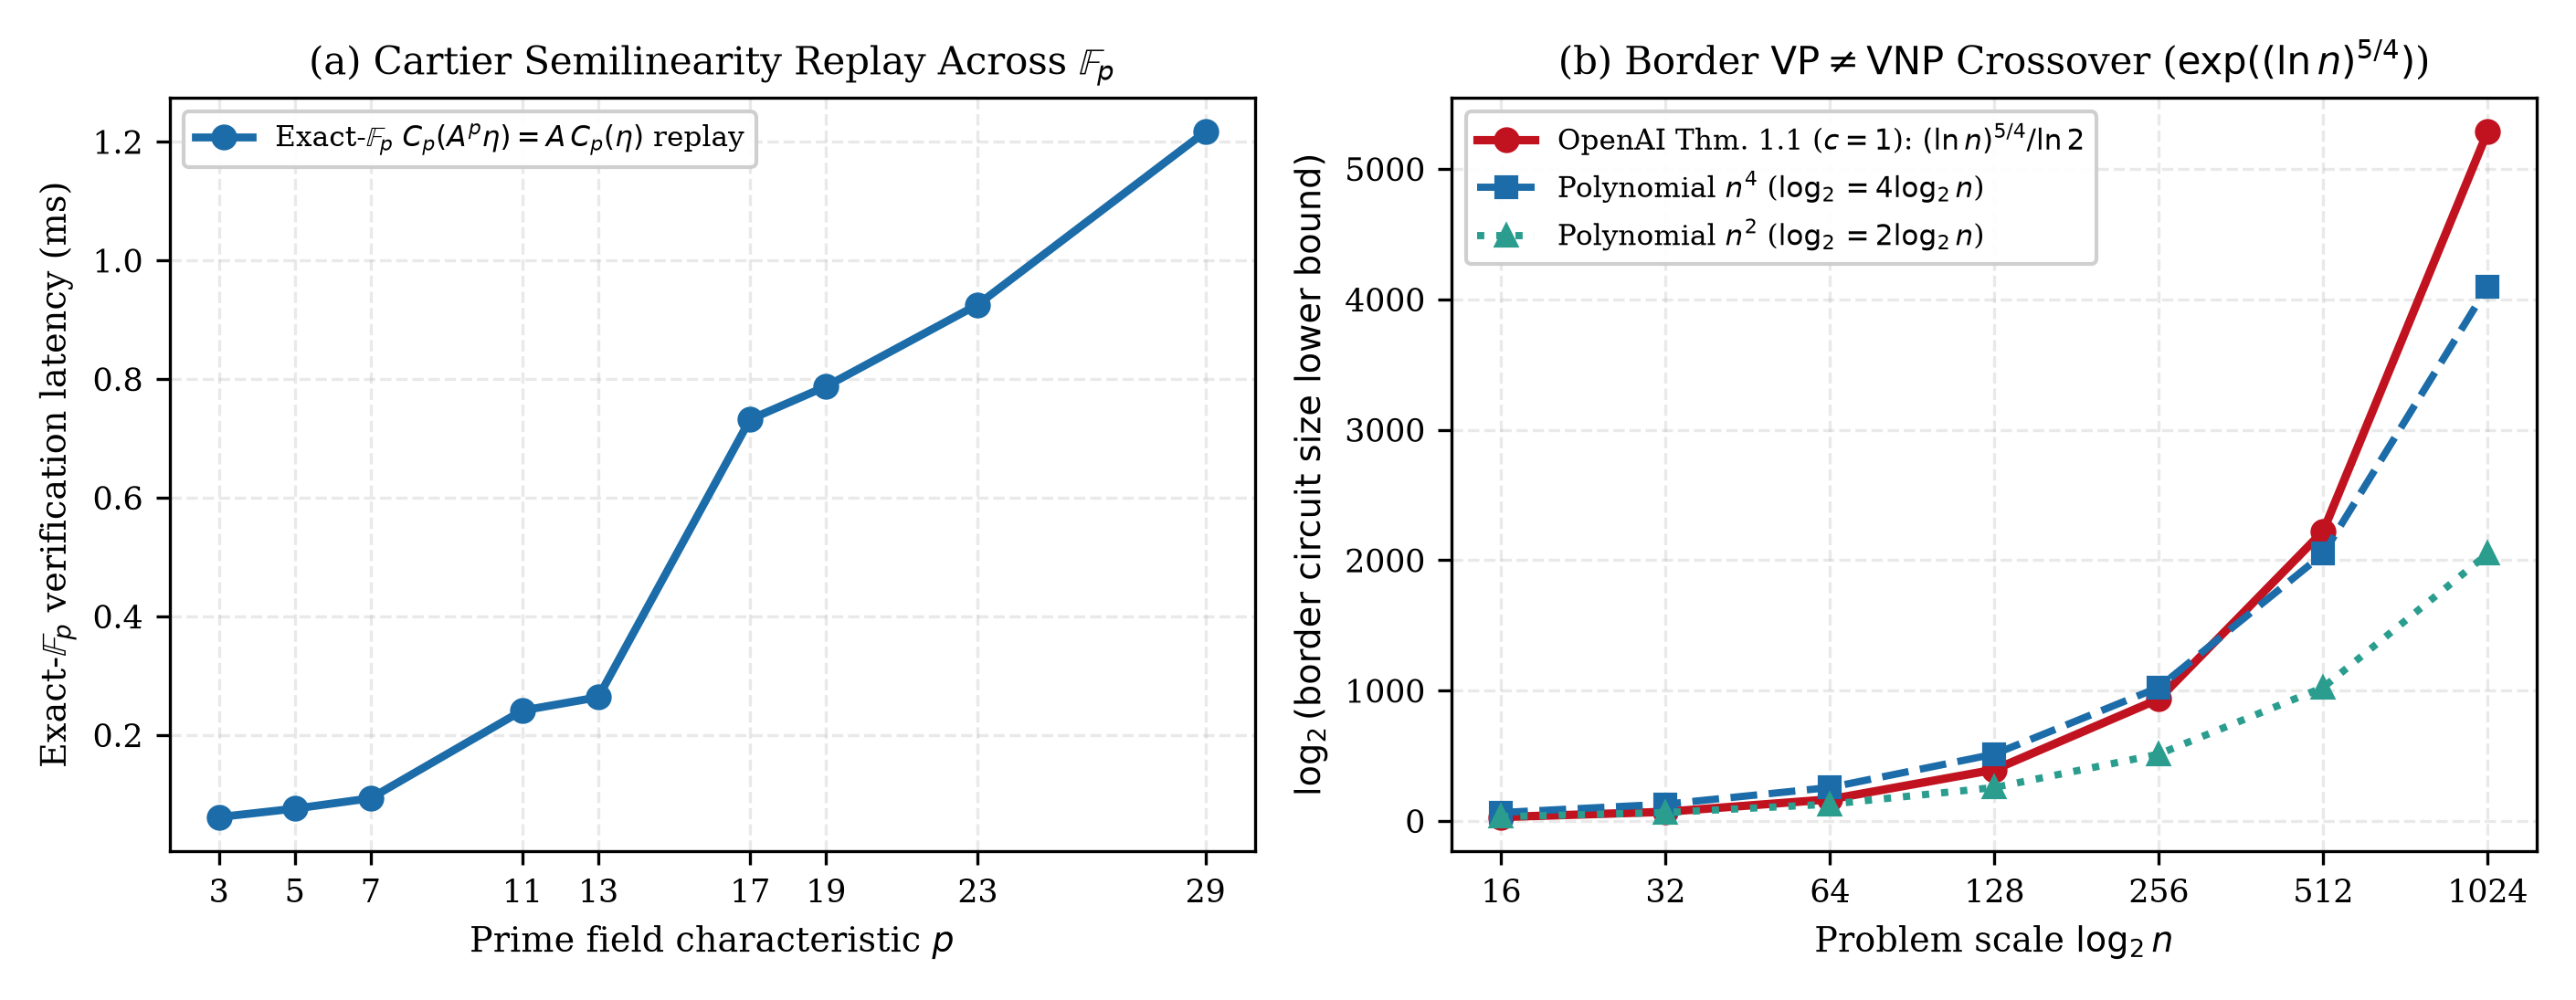
\includegraphics[width=0.90\linewidth]{figures/fig1_cartier_and_crossover.png}
\caption{Cartier replay and border crossover. (a)~Exact-$\FF_p$ Cartier semilinearity replay latency across primes $p = 3\dots 29$. (b)~OpenAI Theorem~1.1 border circuit lower bound $\exp((\ln n)^{5/4})$ ($c=1$) overtaking fixed polynomials $n^2, n^4$.}
\label{fig:cartier}
\end{figure}

\begin{figure}[t!]
\centering
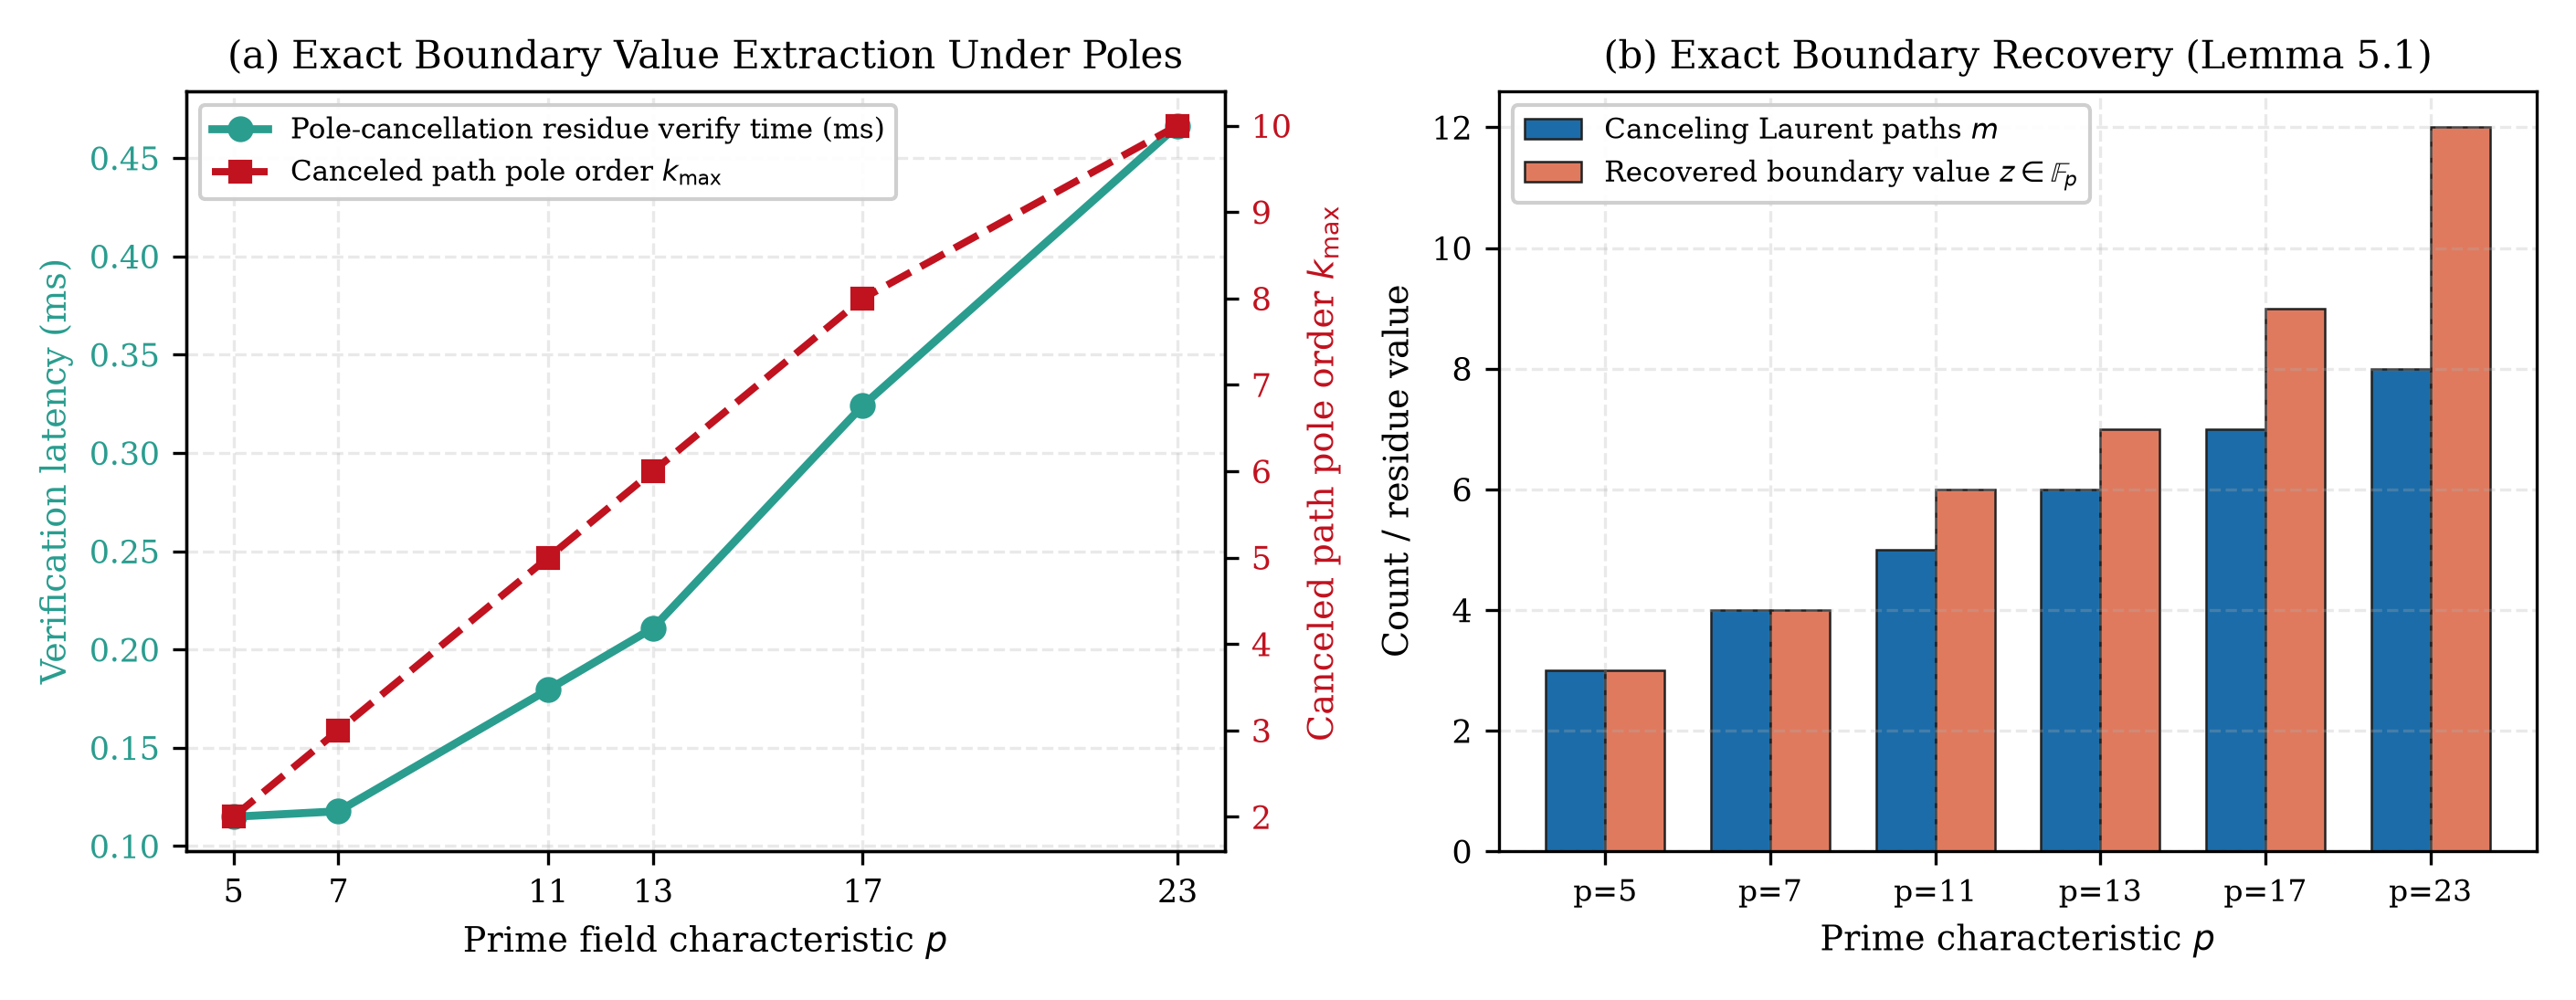
\includegraphics[width=0.90\linewidth]{figures/fig2_pole_cancellation.png}
\caption{Boundary value extraction under cancelling poles (Lemma~5.1). (a)~Exact verification latency and maximal canceled path pole order $k_{\max} = 2\dots 10$ across $p = 5\dots 23$. (b)~Number of cancelling Laurent paths $m$ and recovered boundary values $z \in \FF_p$.}
\label{fig:poles}
\end{figure}

\begin{figure}[t!]
\centering
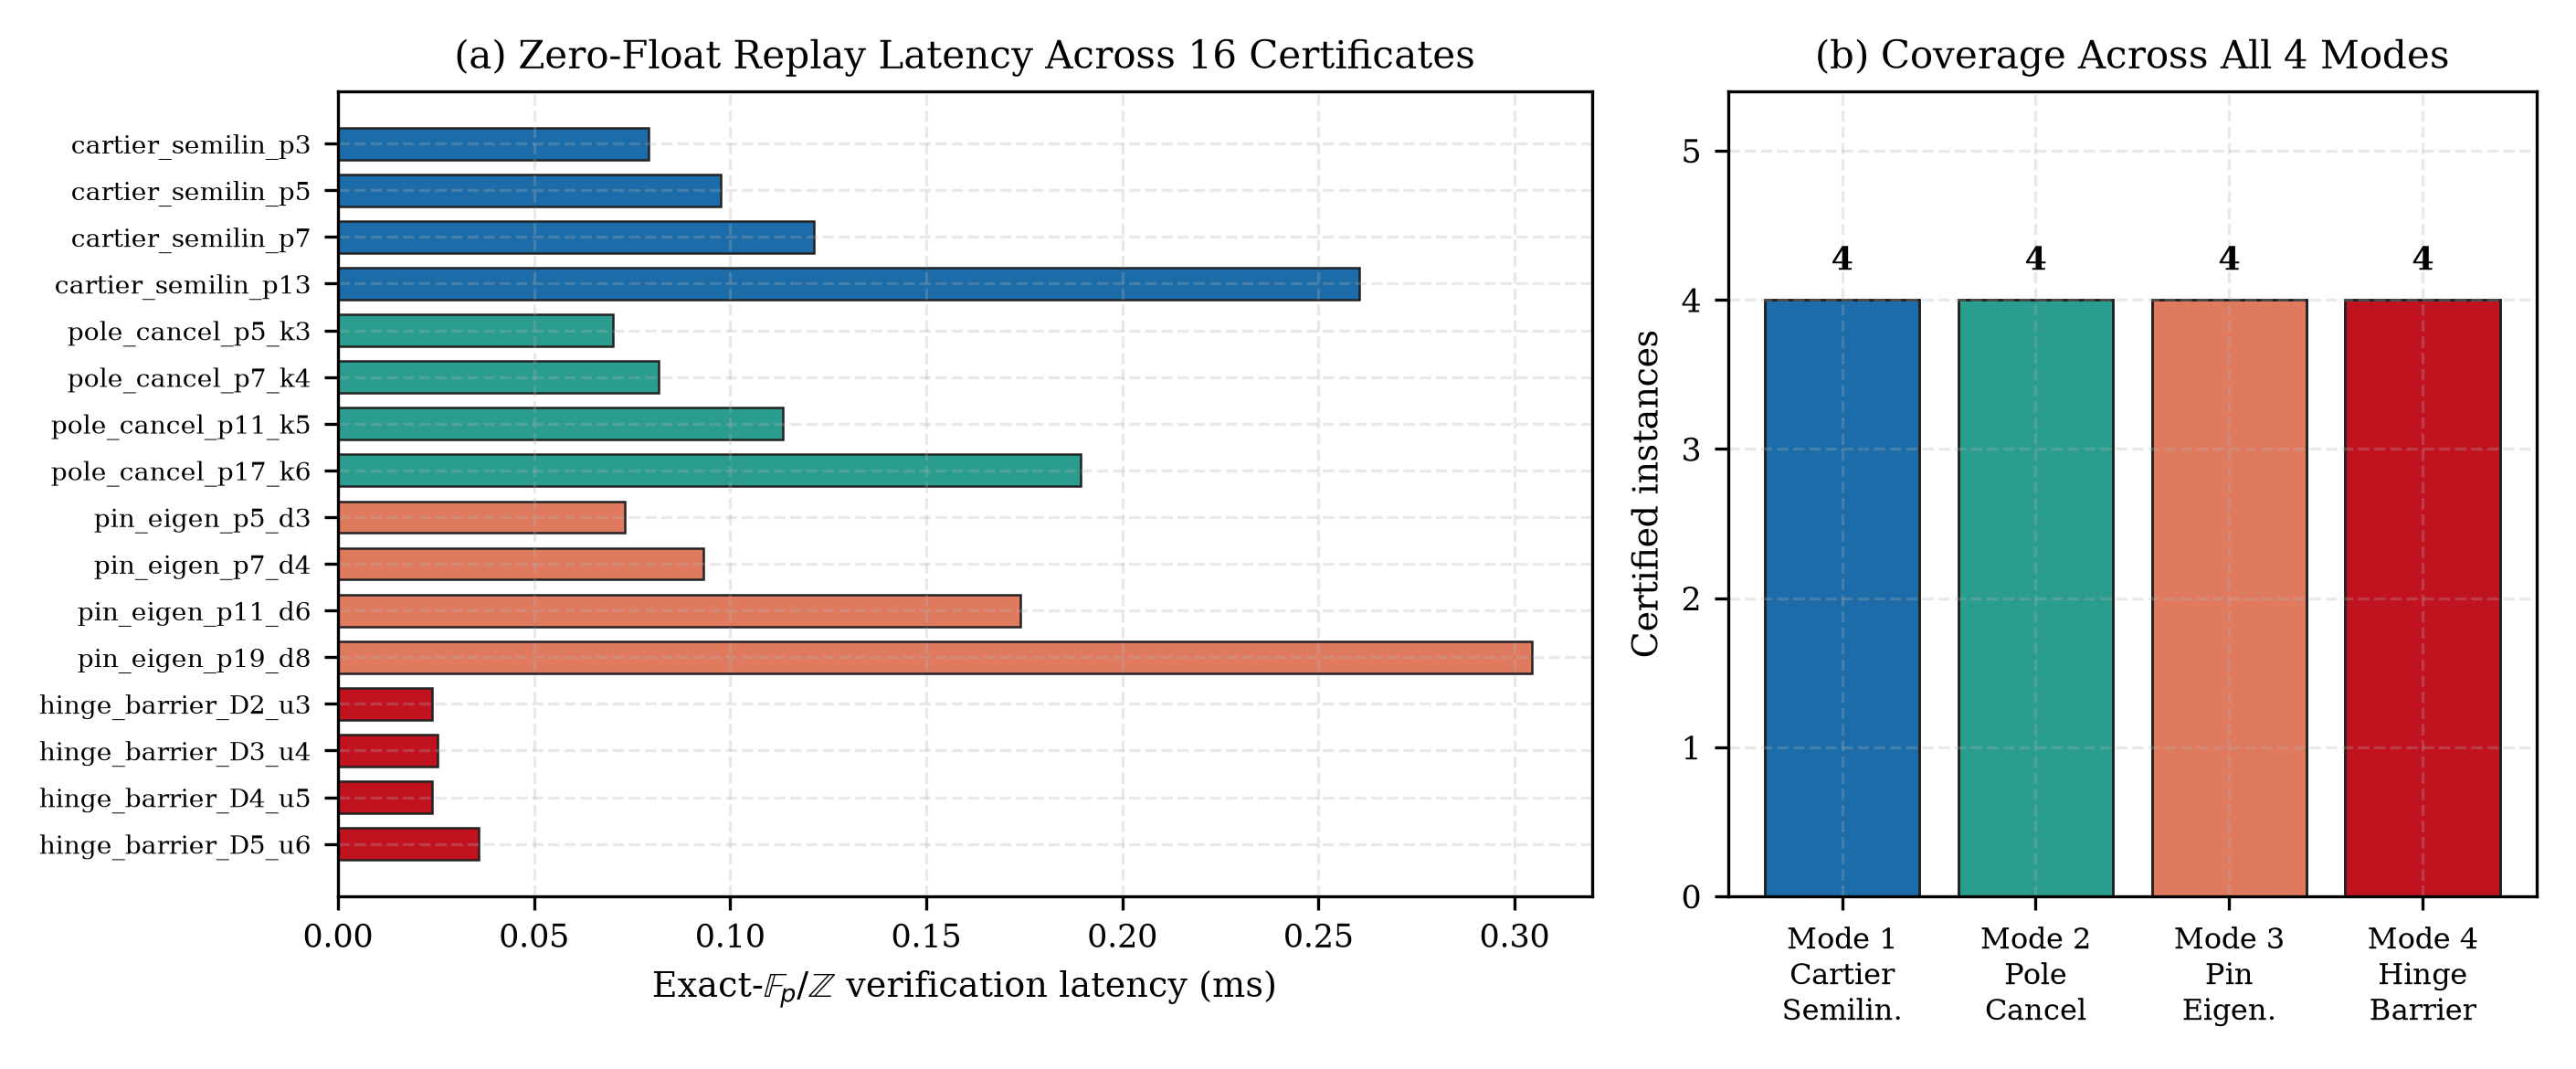
\includegraphics[width=0.90\linewidth]{figures/fig3_atlas_summary.png}
\caption{Certified atlas performance. (a)~Zero-float exact-$\FF_p/\ZZ$ replay latencies across all $16$ \certschema{} certificates ($0.024$--$0.305\,\mathrm{ms}$). (b)~Balanced coverage ($4$ instances per mode) across all four certification modes.}
\label{fig:atlas}
\end{figure}

\section{Scope Boundaries and Outlook}\label{sec:outlook}

This work certifies finite-order characteristic-$p$ Cartier semilinearity, Laurent pole-cancellation boundary extraction, finite-dimensional residue pin eigenvector systems, and hinge/Hadamard/exponent inequalities over $\FF_p$ and $\ZZ$, rather than formalizing the full curve-slicing Zariski-closure geometry, ribbon-host routing, or universal-machine diagonalization of~\cite{openai2026vpvnp}. Extending \certschema{} to multivariate St\"ohr--Voloch Cartier differentials over finite extensions $\FF_{p^r}$ is a natural next step.

\bibliographystyle{plain}
\bibliography{references}

\end{document}
